\section{Grover-Rudolph State Preparation}
\label{sec:grover-rudolph}

In this section, we will describe the Grover-Rudolph state-preparation routine \cite{grover2002creating} in the context that it is used in this work.
The Grover-Rudolph state-preparation algorithm constructs quantum circuits that prepare states of the form given by:
\begin{equation}
    \ket{0^{\otimes \lceil \log_2{L} \rceil}} \rightarrow_{\textit{Grover-Rudolph}} \sum_{l=0}^L \sqrt{p(l)} \ket{l}
\end{equation}
where $p(l)$ is a probability distribution along the different indices ($l$) with the constraint that $\sum_l p(l) = 1$.

In the context of block-encodings, preparing such probability distributions can be used to construct the $Prepare$ oracle:
\begin{equation}
    \ket{0^{\otimes \lceil \log_2{L} \rceil}} \rightarrow_{\textit{Prepare}} \sum_{l = 0}^{L-1} \sqrt{|\alpha_l| / \lambda_{asp}} \ket{l}
\end{equation}
where the probability distribution is defined by the normalized magnitudes of the coefficients of the terms in the linear combination: $p(l) = |\alpha_l| / \lambda_{asp}$.

The Grover-Rudolph algorithm works by sequentially summing up the probability distribution to the left and right of a given index and then performing a rotation controlled based on the current index.

For example, given the coefficients $\alpha_0$, $\alpha_1$, $\alpha_2$, and $\alpha_3$, the Grover-Rudolph algorithm proceeds as follows:
\begin{enumerate}
    \item Perform a Pauli-Y rotation on the top (left-most) qubit in the register by an angle: $\theta = 2 \cos^{-1}\big( \sqrt{\alpha_0 + \alpha_1} \big)$.
    \item Perform a Pauli-Y rotation on the second qubit in the register, controlled on the first qubit being in the state $\ket{0}$ by an angle: $\theta = 2 \cos^{-1}\big( \sqrt{\frac{\alpha_0}{\alpha_0 + \alpha_1}} \big)$
    \item Perform a Pauli-Y rotation on the second qubit in the register, controlled on the first qubit being in the state $\ket{1}$ by an angle: $\theta = 2 \cos^{-1}\big( \sqrt{\frac{\alpha_2}{\alpha_2 + \alpha_3}} \big)$
\end{enumerate}

The evolution of the quantum state is described by:
\begin{equation}
    \begin{split}
        \ket{00} &\rightarrow_{\textit{(i)}} \sqrt{\alpha_0 + \alpha_1} \ket{00} + \sqrt{\alpha_2 + \alpha_3} \ket{10} \\
        &\rightarrow_{\textit{(ii)}} \sqrt{\alpha_0} \ket{00} + \sqrt{\alpha_1} \ket{01} + \sqrt{\alpha_2 + \alpha_3} \ket{10} \\
        &\rightarrow_{\textit{(iii)}} \sqrt{\alpha_0} \ket{00} + \sqrt{\alpha_1} \ket{01} + \alpha_2 \ket{10} + \alpha_3 \ket{11}
    \end{split}
\end{equation}

In Figure \ref{fig:grover-rudolph} a, we show how implementing Grover-Rudolph can be viewed as a series of multiplexed rotations that sequentially act on the next qubit while indexing over the preceeding qubits in the register being prepared.
Prior works \cite{mottonen2004transformation, low2021halving} have shown that multiplexed rotations can be implemented more efficiently than other multiplexed operations by classically preprocessing the rotation angles. 
In Figure \ref{fig:grover-rudolph} b, we show how implementing Grover-Rudolph using the decomposition for multiplexed rotations of \cite{mottonen2004transformation} leads to requiring $L-1$ uncontrolled rotations when preparing $L$ coefficients.
\ws{This value of $L-1$ rotations is certainly true when $L$ is a power of 2. It's not clear that when some of the rotation angles are zero before the classical preprocessing that this cost will still be $L-1$ rotations and not the next highest power of 2.}

\begin{figure}
    \centering
    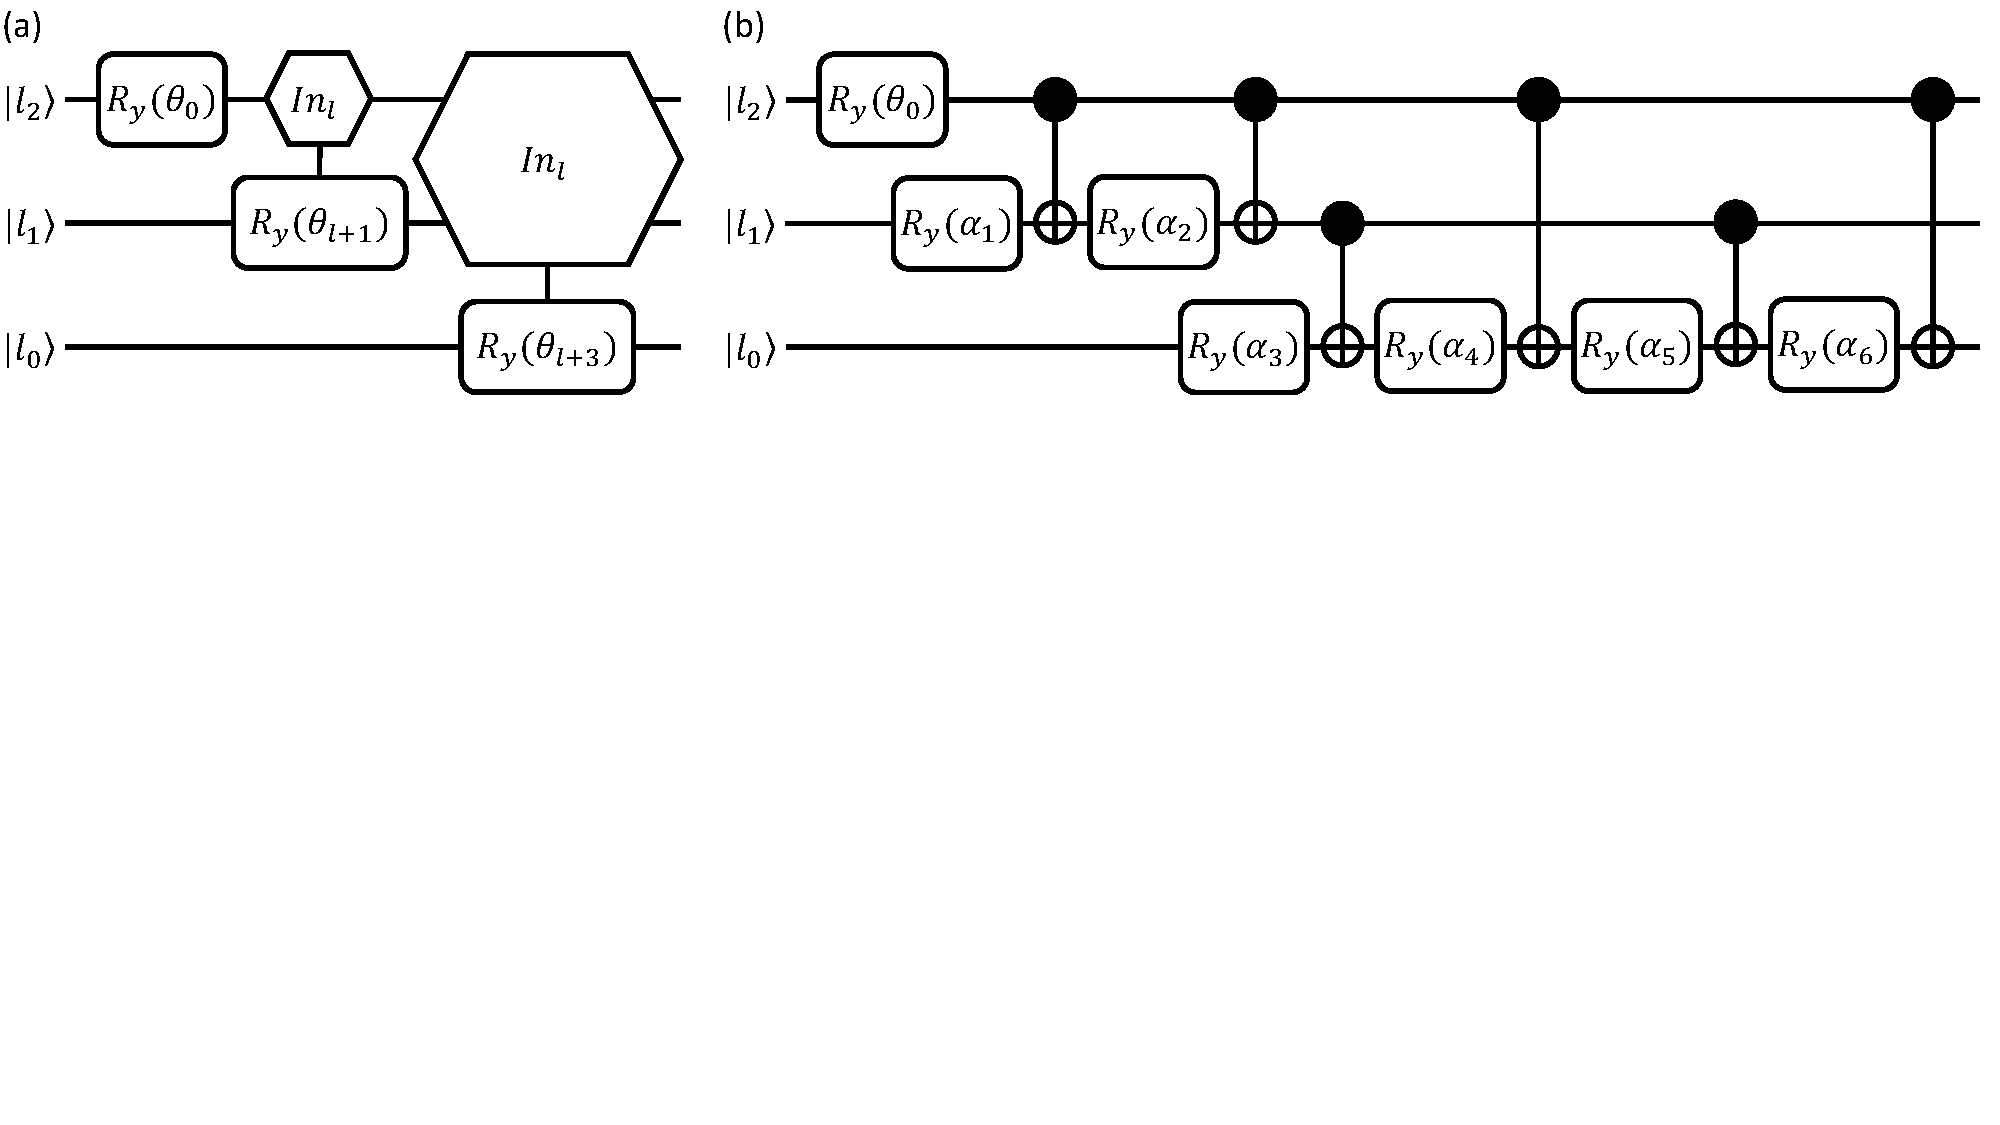
\includegraphics[width=16cm]{figures/grover-rudolph.pdf}
    % 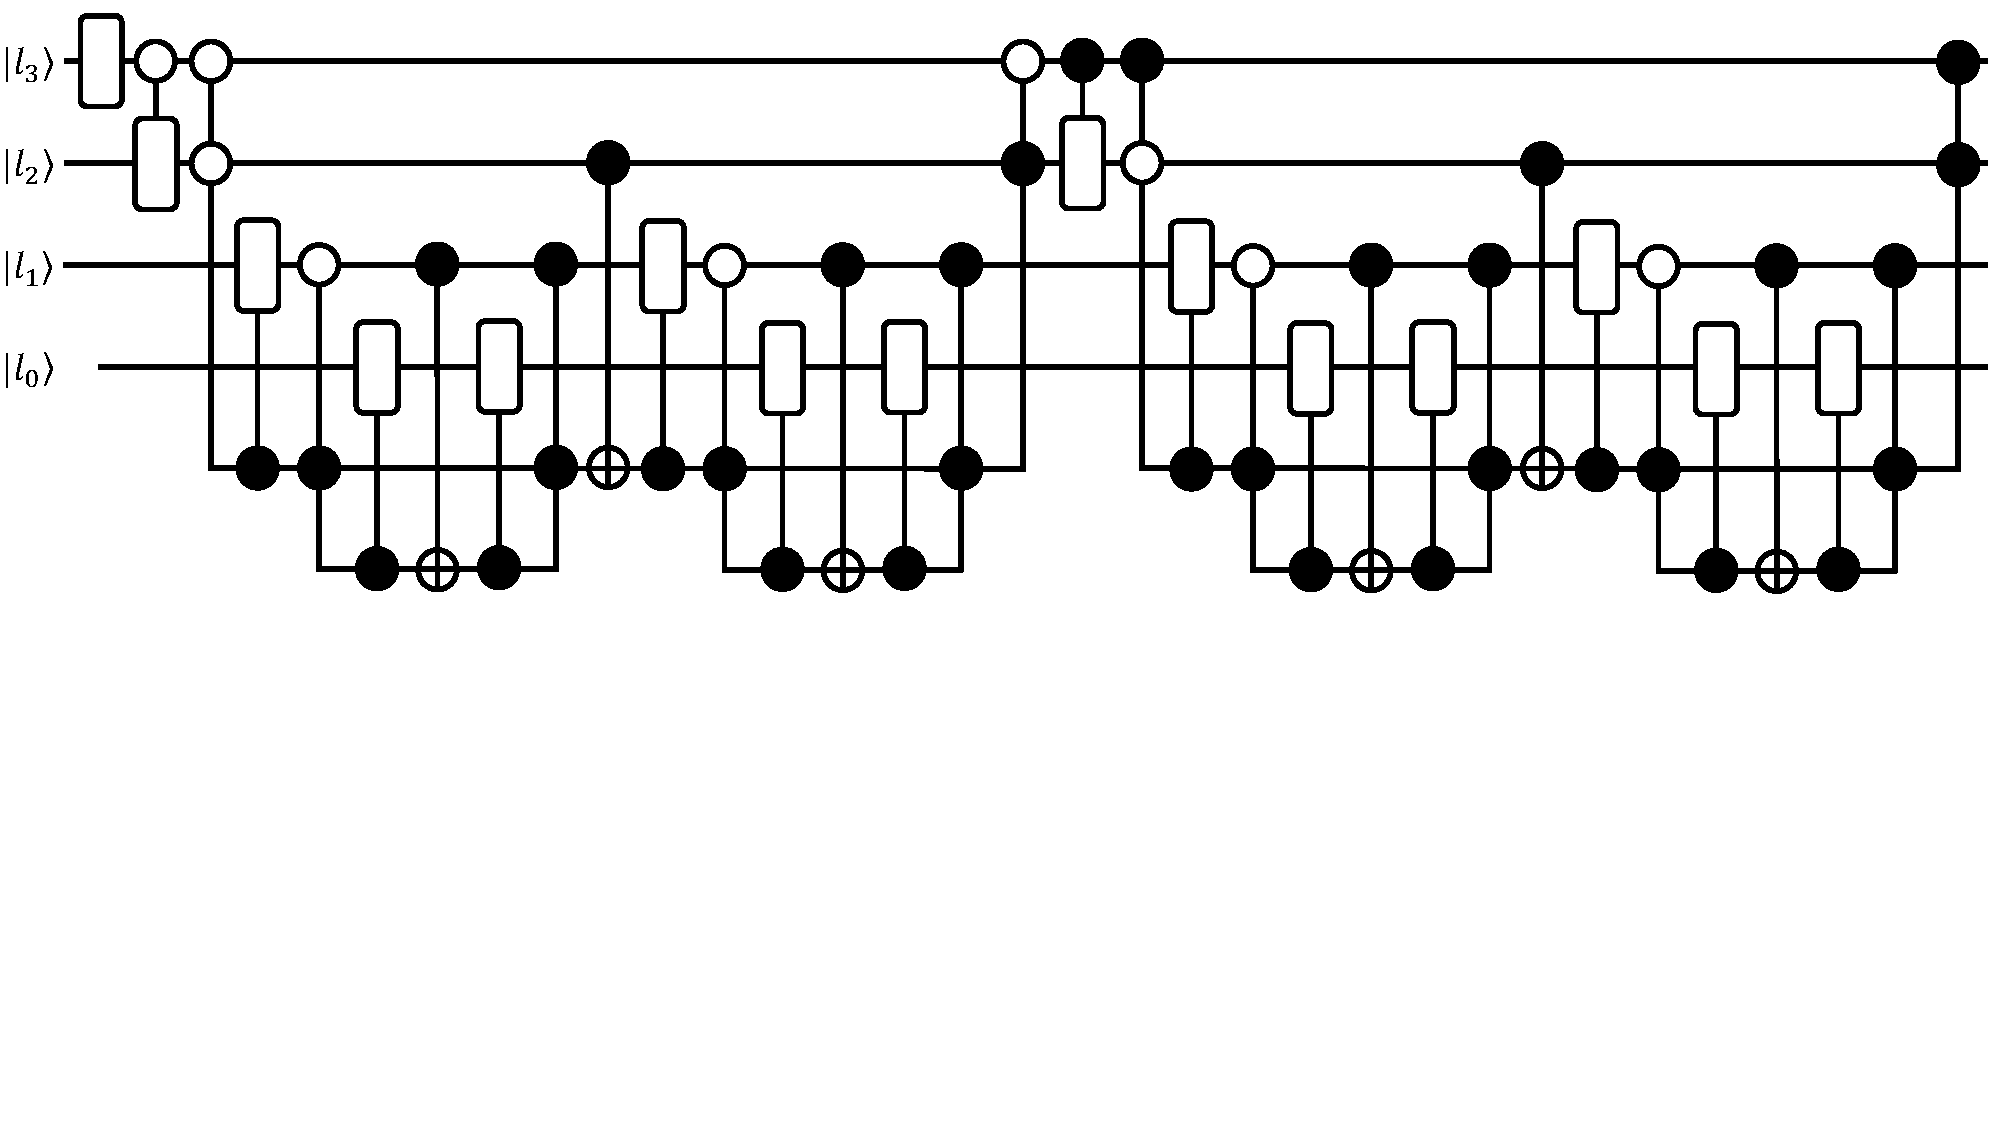
\includegraphics[width=16cm]{figures/grover-rudolph-4-qubits.pdf}
    \caption{
        \textbf{Grover-Rudolph Circuit Compilation.} 
        This figure shows an implementation of the Grover-Rudolph algorithm using multiplexed rotations when preparing 8 coefficients.
        The left subfigure shows the circuit diagram explicitly written as multiplexors, while the right subfigure shows the circuit when the multiplexed rotations are decomposed via \cite{mottonen2004transformation}.
        This circuit requires 7 rotations and the angles of the rotations are changed ($\theta_i \rightarrow \alpha_i$) based on classical preprocessing.
    }
    \label{fig:grover-rudolph}
\end{figure}
